\chapter{ Marco Metodol\'{o}gico}
	
	\section{Metodolog\'{i}a de investigaci\'{o}n}
	
		\subsection{Investigaci\'{o}n-Acci\'{o}n}
	\cite{Baskerville} define la Investigaci\'{o}n-Acci\'{o}n como un m\'{e}todo de investigaci\'{o}n que a finales de la d\'{e}cada de los 90 empez\'{o} a crecer en popularidad, para el uso en investigaciones acad\'{e}micas de sistemas de informaci\'{o}n. Este m\'{e}todo produce resultados de investigaci\'{o}n altamente relevantes debido a que se fundamenta en la acci\'{o}n pr\'{a}ctica, dirigida a resolver un problema mientras se informa cuidadosamente sobre la teor\'{i}a.

	Esta metodolog\'{i}a tiene una doble finalidad: generar un beneficio al cliente de la investigaci\'{o}n y al mismo tiempo generar conocimiento relevante. Por lo tanto, es una forma de investigar de car\'{a}cter colaborativo que busca unir teor\'{i}a y la pr\'{a}ctica entre investigadores y practicantes, mediante un proceso de naturaleza c\'{i}clica.

	La representaci\'{o}n m\'{a}s habitual de la Investigaci\'{o}n-Acci\'{o}n es la descrita por \cite{Baskerville}, en forma de cinco fases que conforman un ciclo, las cuales se muestran en la figura 3.1 y se describen a continuaci\'{o}n.

	\begin{figure}
		\centering
		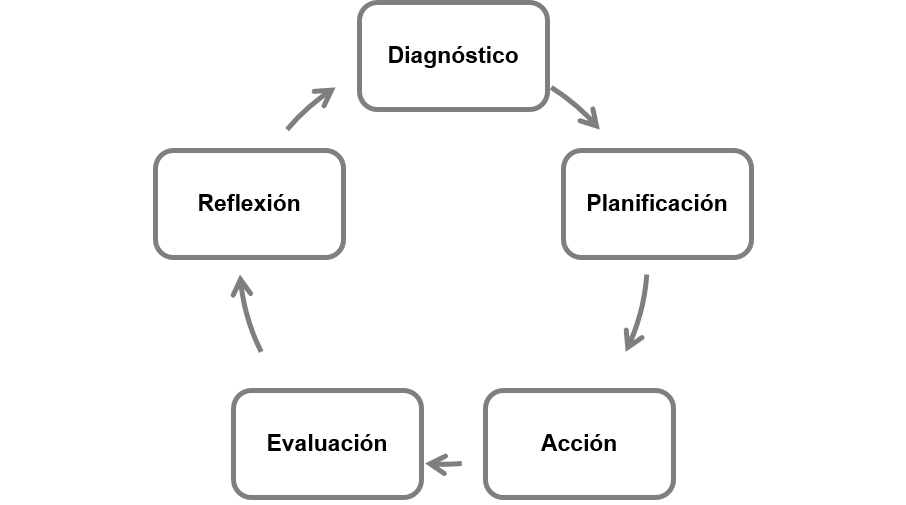
\includegraphics[scale=0.8]{img/investigacion-accion.png}
			\caption[Car\'{a}cter c\'{i}clico de la Investigaci\'{o}n-Acci\'{o}n]{\textit{Car\'{a}cter c\'{i}clico de la Investigaci\'{o}n-Acci\'{o}n} (Fuente: Baskerville, 1999).}
	\end{figure}

	\begin{itemize}
		\item \textbf{Fase de diagn\'{o}stico:} se realiza el proceso de identificaci\'{o}n de los problemas primarios de la investigaci\'{o}n.
		\item \textbf{Fase de planificaci\'{o}n:} se especifican las acciones que se llevar\'{a}n a cabo para solucionar los problemas primarios.
		\item \textbf{Fase de acci\'{o}n:} se ejecutan las acciones planificadas en la fase anterior.
		\item \textbf{Fase de evaluaci\'{o}n u observaci\'{o}n:} se efect\'{u}a una evaluaci\'{o}n de los resultados obtenidos para observar, conocer y documentar los efectos de las acciones que fueron realizadas.
		\item \textbf{Fase de reflexi\'{o}n:} se toman los conocimientos adquiridos en la Investigaci\'{o}n-Acci\'{o}n. Si las acciones ejecutadas no fueron exitosas, los conocimientos pueden proporcionar la base para el diagn\'{o}stico de un nuevo ciclo de Investigaci\'{o}n-Acci\'{o}n.
	\end{itemize}

En la tabla 3.1 se muestran las actividades de la presente investigaci\'{o}n, haciendo correspondencia a cada una de las fases de la Investigaci\'{o}n-Acci\'{o}n descritas por \cite{Baskerville}.

	\begin{table}[t]
		\small
		\caption[Actividades del proyecto seg\'{u}n la Investigaci\'{o}n-Acci\'{o}n]{\textit{Actividades del proyecto seg\'{u}n la Investigaci\'{o}n-Acci\'{o}n} (Fuente: Autor).}
		\centering
		\setlength{\extrarowheight}{\altocelda}
		\begin{tabulary}{\anchotabla}{|c|J|}
			\hline
			\thead{\textbf{\small{Fase}}} & \thead{\textbf{\small{Actividades}}}\\ \hline
			\textbf{Diagn\'{o}stico} & Identificar los problemas y limitaciones que presenta el HunterLab Universal Software.\\ \hline
			\textbf{Planificaci\'{o}n} & Seleccionar la metodolog\'{i}a de desarrollo, determinar los requisitos del software y realizar un plan de trabajo.
\\ \hline
			\textbf{Acci\'{o}n} & Desarrollar el software, tomando en cuenta los requisitos identificados previamente y los lineamientos de calidad del software.\\ \hline
			\textbf{Evaluaci\'{o}n} & Realizar las pruebas de funcionalidad y de usabilidad al software.\\ \hline
			\textbf{Reflexi\'{o}n} & Presentar los resultados y los an\'{a}lisis de las pruebas realizadas.\\ \hline
		\end{tabulary}
	\end{table}

\vspace*{0.5 cm}

	\section{Metodolog\'{i}a de desarrollo de software}
Para que el desarrollo del nuevo software cumpliera con los objetivos propuestos en la presente investigaci\'{o}n, y tomando en cuenta los atributos de calidad planteados por la ingenier\'{i}a del software, se realiz\'{o} una revisi\'{o}n del enfoque que deber\'{i}a tener la metodolog\'{i}a de desarrollo a utilizar.

Seg\'{u}n \cite{Sommerville}, en los a\~{n}os 80 y a principios de los 90, exist\'{i}a una opini\'{o}n general de que la mejor forma de obtener un software de calidad era a trav\'{e}s de una planificaci\'{o}n cuidadosa del proyecto, una garant\'{i}a de calidad formalizada, la utilizaci\'{o}n de m\'{e}todos de an\'{a}lisis y dise\~{n}o soportados por herramientas \textit{CASE}, y por medio de procesos de desarrollo de software controlados y rigurosos. El software que segu\'{i}a lo mencionado previamente era desarrollado por grandes equipos que a veces trabajaban para compa\~{n}\'{i}as diferentes, que a menudo estaban dispersos geogr\'{a}ficamente y trabajaban en el software durante largos periodos de tiempo.

Ahora bien, debido a que se ten\'{i}a un equipo peque\~{n}o para el desarrollo del nuevo software, y a que no se iba a trabajar en \'{e}ste durante un largo periodo de tiempo, se eligi\'{o} la utilizaci\'{o}n de una metodolog\'{i}a de desarrollo de enfoque \'{a}gil. De acuerdo con \cite{Sommerville}, los m\'{e}todos \'{a}giles dependen de un enfoque iterativo para la especificaci\'{o}n, el desarrollo y la entrega del software, y est\'{a}n pensados para entregar un producto funcional de forma r\'{a}pida a los clientes, quienes pueden entonces proponer que se incluyan en iteraciones posteriores nuevos requerimientos o cambios en los mismos. Si bien los m\'{e}todos \'{a}giles proponen procesos diferentes para el desarrollo y entregas incrementales del software, comparten unos principios en com\'{u}n, los cuales son ilustrados en la tabla 3.2.

	\begin{table}[t]
		\small
		\caption[Principios de los m\'{e}todos \'{a}giles]{\textit{Principios de los m\'{e}todos \'{a}giles} (Fuente: Sommerville, 2005).}
		\centering
		\setlength{\extrarowheight}{\altocelda}
		\begin{tabulary}{\anchotabla}{|c|J|}
			\hline
			\thead{\textbf{\small{Principio}}} & \thead{\textbf{\small{Descripci\'{o}n}}}\\ \hline
			\textbf{Participaci\'{o}n del cliente} & Los clientes deben estar fuertemente implicados en todo el proceso de desarrollo.\\ \hline
			\textbf{Entrega incremental} & El software se desarrolla en incrementos, en los que el cliente especifica los requerimientos a incluir en cada incremento.\\ \hline
			\textbf{Personas, no procesos} & Se deben reconocer y explotar las habilidades del equipo de desarrollo. A \'{e}ste se le debe dejar desarrollar su propia forma de trabajar, sin procesos formales.\\ \hline
			\textbf{Aceptar el cambio} & Se debe contar con que los requerimientos del software cambian, por lo que el software se dise\~{n}a para dar cabida a estos cambios.\\ \hline
			\textbf{Mantener la simplicidad} & Se debe centrar la simplicidad tanto en el software a desarrollar como en el proceso de desarrollo. Donde sea posible, se trabaja activamente para eliminar la complejidad del software.\\ \hline
		\end{tabulary}
	\end{table}

		\subsection{SCRUM}
De acuerdo con \cite{Schwaber&Sutherland}, esta metodolog\'{i}a \'{a}gil es un marco de trabajo de procesos, que ha sido utilizado para gestionar el desarrollo de productos complejos desde principios de los a\~{n}os 90. SCRUM muestra la eficacia relativa de las pr\'{a}cticas de gesti\'{o}n de productos y las pr\'{a}cticas de desarrollo.

La estructura de desarrollo de SCRUM se basa en ciclos de trabajo llamados \textit{sprints}. Los \textit{sprints} son iteraciones de una a cuatro semanas que suceden una detr\'{a}s de la otra, con una duraci\'{o}n fija y con fechas de culminaci\'{o}n previamente establecidas. Se seleccionan los requerimientos que se van a desarrollar de una lista priorizada. Todos los d\'{i}as el equipo se re\'{u}ne, y al final del \textit{sprint} el equipo revisa el mismo con los \textit{stakeholders}.

\cite{Hundermark} explica de forma precisa los roles que conforman el equipo de desarrollo de SCRUM, que se detallan a continuaci\'{o}n:
			
		\begin{itemize}
				
				\item \textbf{Due\~{n}o del producto \textit{(Product Owner)}:} su responsabilidad es optimizar el retorno de la inversi\'{o}n, asegurando que el equipo SCRUM este ocupado en entregar las caracter\'{i}sticas m\'{a}s valiosas del producto. Su trabajo principal es concentrarse en la efectividad, esto es elaborar el producto correcto para sus clientes.
				
				\item \textbf{Equipo de desarrollo:} es un grupo de personas responsables por entregar incrementos de la funcionalidad del producto al final de cada \textit{sprint}. El trabajo principal de este equipo es concentrarse en la eficiencia, esto es elaborar el producto correcto para su \textit{Product Owner} y sus usuarios.
				
				\item \textbf{Maestro SCRUM \textit{(SCRUM Master)}:} gestiona todos los aspectos del proceso del equipo SCRUM. Su trabajo principal es concentrarse en el progreso continuo del equipo, acortando los ciclos de retroalimentaci\'{o}n mediante los cuales aprende.
				
		\end{itemize}
			
			Como es sabido, el \textit{sprint} marca cada una de las iteraciones dentro del ciclo de desarrollo de SCRUM. Por otra parte, la planificaci\'{o}n, la continua revisi\'{o}n y la retrospectiva definen el inicio y el final del \textit{sprint}. Las reuniones que ocurren en cada \textit{sprint} son las siguientes.
			
			\begin{itemize}
				\item \textbf{Reuni\'{o}n de planificaci\'{o}n del \textit{sprint}: }
				esta reuni\'{o}n marca el inicio de cada \textit{sprint}. Su prop\'{o}sito para el equipo SCRUM es planear el trabajo que van a realizar durante el \textit{sprint} actual.
				
				\item \textbf{Reuni\'{o}n diaria del \textit{sprint}: }
				el equipo de desarrollo se reune para comunicar su trabajo, sincronizarlo y crear un plan para las siguientes 24 horas. Esta colaboraci\'{o}n es esencial para asegurar el progreso continuo y evadir cualquier obstrucci\'{o}n de trabajo.
				
				\item \textbf{Reuni\'{o}n de revisi\'{o}n del \textit{sprint}: }
				su prop\'{o}sito es el de inspeccionar la iteraci\'{o}n del producto que el equipo de desarrollo ha entregado, obtener una retroalimentaci\'{o}n de los participantes en la reuni\'{o}n con respecto a la misma, y adaptar el plan para el \textit{sprint} subsiguiente. Esta reuni\'{o}n est\'{a} abierta para todo el personal dentro de la organizaci\'{o}n.
				
				\item \textbf{Reuni\'{o}n de retrospectiva: }
				es la reuni\'{o}n final del \textit{sprint}, la cual nunca es omitida, sin importar lo que haya ocurrido en dicho \textit{sprint}. Mientras que la reuni\'{o}n de revisi\'{o}n del \textit{sprint} est\'{a} enfocada en el producto, esta reuni\'{o}n est\'{a} enfocada en el proceso, es decir, la forma en la que el equipo SCRUM est\'{a} trabajando en conjunto, incluyendo sus habilidades t\'{e}cnicas, las pr\'{a}cticas de desarrollo del software y las herramientas que est\'{a}n usando. Esta reuni\'{o}n se limita a los miembros del equipo SCRUM.
				
			\end{itemize}
			
Por otra parte, la metodolog\'{i}a SCRUM incluye los siguientes artefactos:
			
			\begin{itemize}
				\item \textbf{Pila del producto \textit{(product backlog)}: }
					es una lista de \'{i}tems de trabajo descritos en un nivel funcional, que necesitan ser realizados a lo largo del tiempo. Los requerimientos son emergentes, lo que significa que no se puede saber por adelantado todos los detalles acerca de lo que se quiere en el producto. Por esta raz\'{o}n este artefacto es un documento din\'{a}mico, que requiere un refinamiento constante para mantenerlo actual y \'{u}til.
				
				\item \textbf{Pila del \textit{sprint} \textit{(sprint backlog)}: }
				esta pila es visualizada por el equipo de desarrollo en un \textit{task board}, que es la representaci\'{o}n f\'{i}sica de la lista de trabajo que se ha resumido para realizar durante el \textit{sprint} actual. Este artefacto le dice al equipo SCRUM y a todos los dem\'{a}s el trabajo que tienen planeado hacer en el \textit{sprint}, y su estado actual.
				
				\item \textbf{Incremento: }
				es la suma de todos los \'{i}tems de la pila del producto que cumplen con la definici\'{o}n de terminado al final del \textit{sprint}. El equipo de desarrollo presentar\'{a} el incremento en la revisi\'{o}n del \textit{sprint}, y el \textit{Product Owner} determinar\'{a} cu\'{a}ndo liberarlo.
				
			\end{itemize}
			
En esta metodolog\'{i}a se pueden emplear varias t\'{e}cnicas y procesos. En este sentido, se incluyeron algunos artefactos de la metodolog\'{i}a RUP (\textit{Rational Unified Process}) descrita por \cite{Kroll&Kruchten}, para as\'{i} generar suficiente documentaci\'{o}n durante el dise\~{n}o y el desarrollo del software. 

	\subsection{Artefactos de RUP utilizados}
	
		\begin{itemize}
			\item \textbf{Documento de visi\'{o}n: }describe la visi\'{o}n de los \textit{stakeholders} con respecto al producto a desarrollarse, especificado en t\'{e}rminos de las caracter\'{i}sticas y las necesidades claves de los mismos.
			
			\item \textbf{Modelo de casos de uso: }describe los requerimientos funcionales del software en t\'{e}rminos de actores y casos de uso. Un actor representa el tipo de usuario del software, mientras que un caso de uso describe c\'{o}mo va a interactuar cada actor con el software.
			
			\item \textbf{Requerimientos no funcionales: } representan los requerimientos que tienen un impacto significativo en la arquitectura y en la satisfacci\'{o}n del usuario.
			
			\item \textbf{Glosario: }define la terminolog\'{i}a empleada en todos los artefactos utilizados.
		\end{itemize}

\newpage

Para finalizar, en la figura 3.2 se ilustra la configuraci\'{o}n de la metodolog\'{i}a SCRUM utlizada, en conjunto con los artefactos elegidos de la metodolog\'{i}a RUP.
	
	\FloatBarrier
	\begin{figure}[h]
		\centering
		
\includegraphics[scale=0.8]{img/SCRUM-RUP.png}
			\caption[Configuraci\'{o}n de los artefactos a utilizar de SCRUM y RUP]{\textit{Configuraci\'{o}n de los artefactos a utilizar de SCRUM y RUP} (Fuente: Autor).}
	\end{figure}
	\FloatBarrier
	